\chapter{Gestion des habilitations -- principes retenus pour le logiciel Collec}
\label{oauth}

Le mécanisme d'identification prévu pour les services web s'appuie en grande partie sur le protocole OAuth v2, au moins dans ses principes. Ce n'est pas le protocole qui est effectivement implémenté (OAuth est prévu pour que l'utilisateur définisse les droits d'accès de l'application cliente), mais les principes d'identification retenus s'en inspirent.

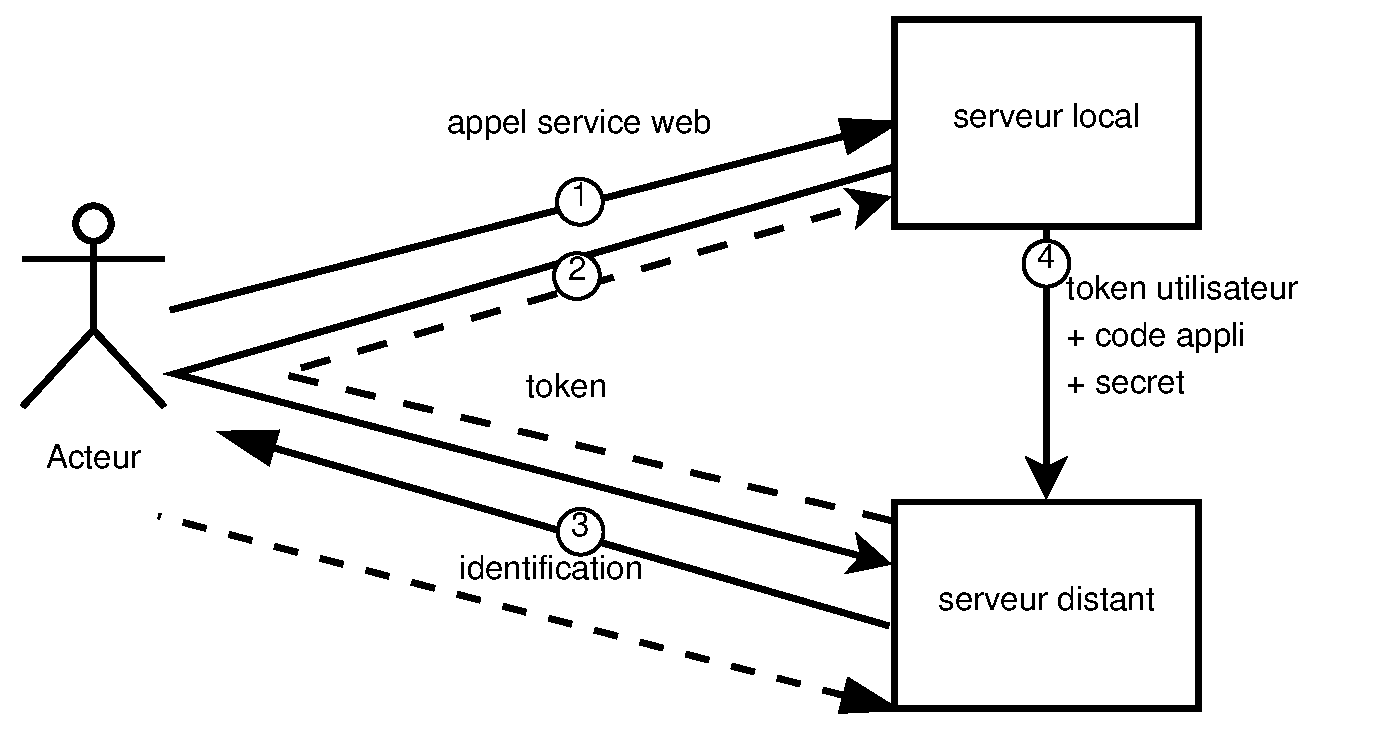
\includegraphics[width=\linewidth]{images/appel_sw_identification}

Pour accéder à des informations distantes, le dialogue entre les deux serveurs nécessite plusieurs phases :
\begin{enumerate}
\item l'utilisateur veut déclencher l'appel à un service web distant ;
\item aucun jeton n'a été récupéré par le serveur local : l'utilisateur est redirigé vers le serveur distant pour obtenir un jeton d'identification;
\item le serveur distant ne connaît pas l'utilisateur : il lui demande de s'identifier en utilisant la procédure adéquate (\textit{login/mot de passe} dans la plupart des cas);
\\une fois identifié, le serveur distant renvoie le navigateur de l'utilisateur vers le serveur local, en fournissant un jeton chiffré;
\item l'appel au service web peut maintenant être déclenché, en fournissant:
\begin{itemize}
\item le jeton de l'utilisateur;
\item le code de l'application locale;
\item le secret partagé entre l'application distante et l'application locale.
\end{itemize}
\end{enumerate}


\section{Opérations préalables à l'interrogation d'une \\base de données distante}
\subsection{Identification réciproque des applications}

Les applications clientes doivent se faire identifier par les applications distantes avant tout échange.

Cette étape est manuelle : l'administrateur de l'application distante crée un enregistrement dans la table \textit{instance}, dont le détail est décrit dans la section \ref{table_instance}.

Le code d'identification, ainsi que le secret associé, est envoyé par mail (de manière automatique ou semi-automatique de préférence) par l'administrateur de la base distante (\textit{cf.} section \ref{dist_record}).

Ces informations sont stockées dans la table \textit{instance} locale, en indiquant en outre les adresses des différents services web disponibles pour le serveur distant.

\subsection{Identification des utilisateurs}
Les utilisateurs qui peuvent utiliser les services web distants sont enregistrés dans le serveur distant et disposent d'un code d'identification. Une fois connectés, ils doivent hériter du droit \textit{consultsw}, indispensable pour accéder aux services web.

Pour qu'ils puissent récupérer les données \og métier \fg{}, les utilisateurs doivent également être rattachés à un projet. Dans la pratique, dans la gestion des groupes de logins, on trouvera l'arborescence suivante (par exemple):
\begin{center}

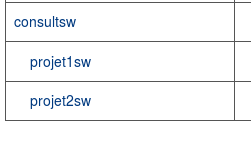
\includegraphics[width=5cm]{images/arborescence_groupes_sw}

\end{center}

Les utilisateurs distants sont associés aux groupes \textit{projet1sw} ou \textit{projet2sw}, et ces groupes sont associés aux projets (ou sous-collections) adéquats pour leur donner les droits d'accès en lecture.